\documentclass[a4paper,12pt]{revtex4}
\usepackage[paperwidth=210mm, paperheight=297mm, margin=2.5cm]{geometry}
\usepackage[none]{hyphenat}
\usepackage{amsmath}
\usepackage{graphicx}
\usepackage{hyperref}
\usepackage{array}
\usepackage{booktabs}
\usepackage{amssymb}
\usepackage{physics}
\usepackage{tikz}
\usetikzlibrary{arrows.meta}
\usepackage{pgfplots}
\pgfplotsset{compat=1.18}
\usetikzlibrary{arrows.meta}

\sloppy
\begin{document}
\author{Omar Iskandarani}
\title{Tijdsdilatatie in een 3D Superfluïde Æther Model, Gebaseerd op Wervel kernrotatie en ætherische Stroom}
\date{\today}
\affiliation{Onafhankelijk onderzoeker, Groningen, Nederland}
\thanks{ORCID: \href{https://orcid.org/0009-0006-1686-3961}{0009-0006-1686-3961}}
\email{info@omariskandarani.com}

\maketitle

\section*{Abstract}
In dit artikel leiden we tijdsdilatatievergelijkingen af binnen een 3D Euclidisch superfluïde æthermodel. In het Vortex-Æther Model (VAM) beschouwen we een \textit{wervel} (vortex) als een topologisch behouden draaiveld in een superfluïde medium. In dit raamwerk worden fundamentele deeltjes gemodelleerd als wervelknopen en wordt tijd gedefinieerd door de intrinsieke hoekrotatie van hun wervelkernen. Het doel is om het ruimtetijdkrommingsconcept van de algemene relativiteitstheorie (GR) te vervangen door gekwantiseerde hoeksnelheidsvelden in een vlakke-ruimte-æther, terwijl alle experimentele voorspellingen van tijdsdilatatie onder GR en speciale relativiteitstheorie (SR) worden gereproduceerd. We bieden afleidingen van eerste principes, gegrond in vloeistofdynamica en wervelmechanica, en drukken de tijdsdilatatiefactoren uit in termen van fundamentele constanten zoals de Planck-tijd en maximale kracht.




\begin{figure}[htbp]
    \centering
    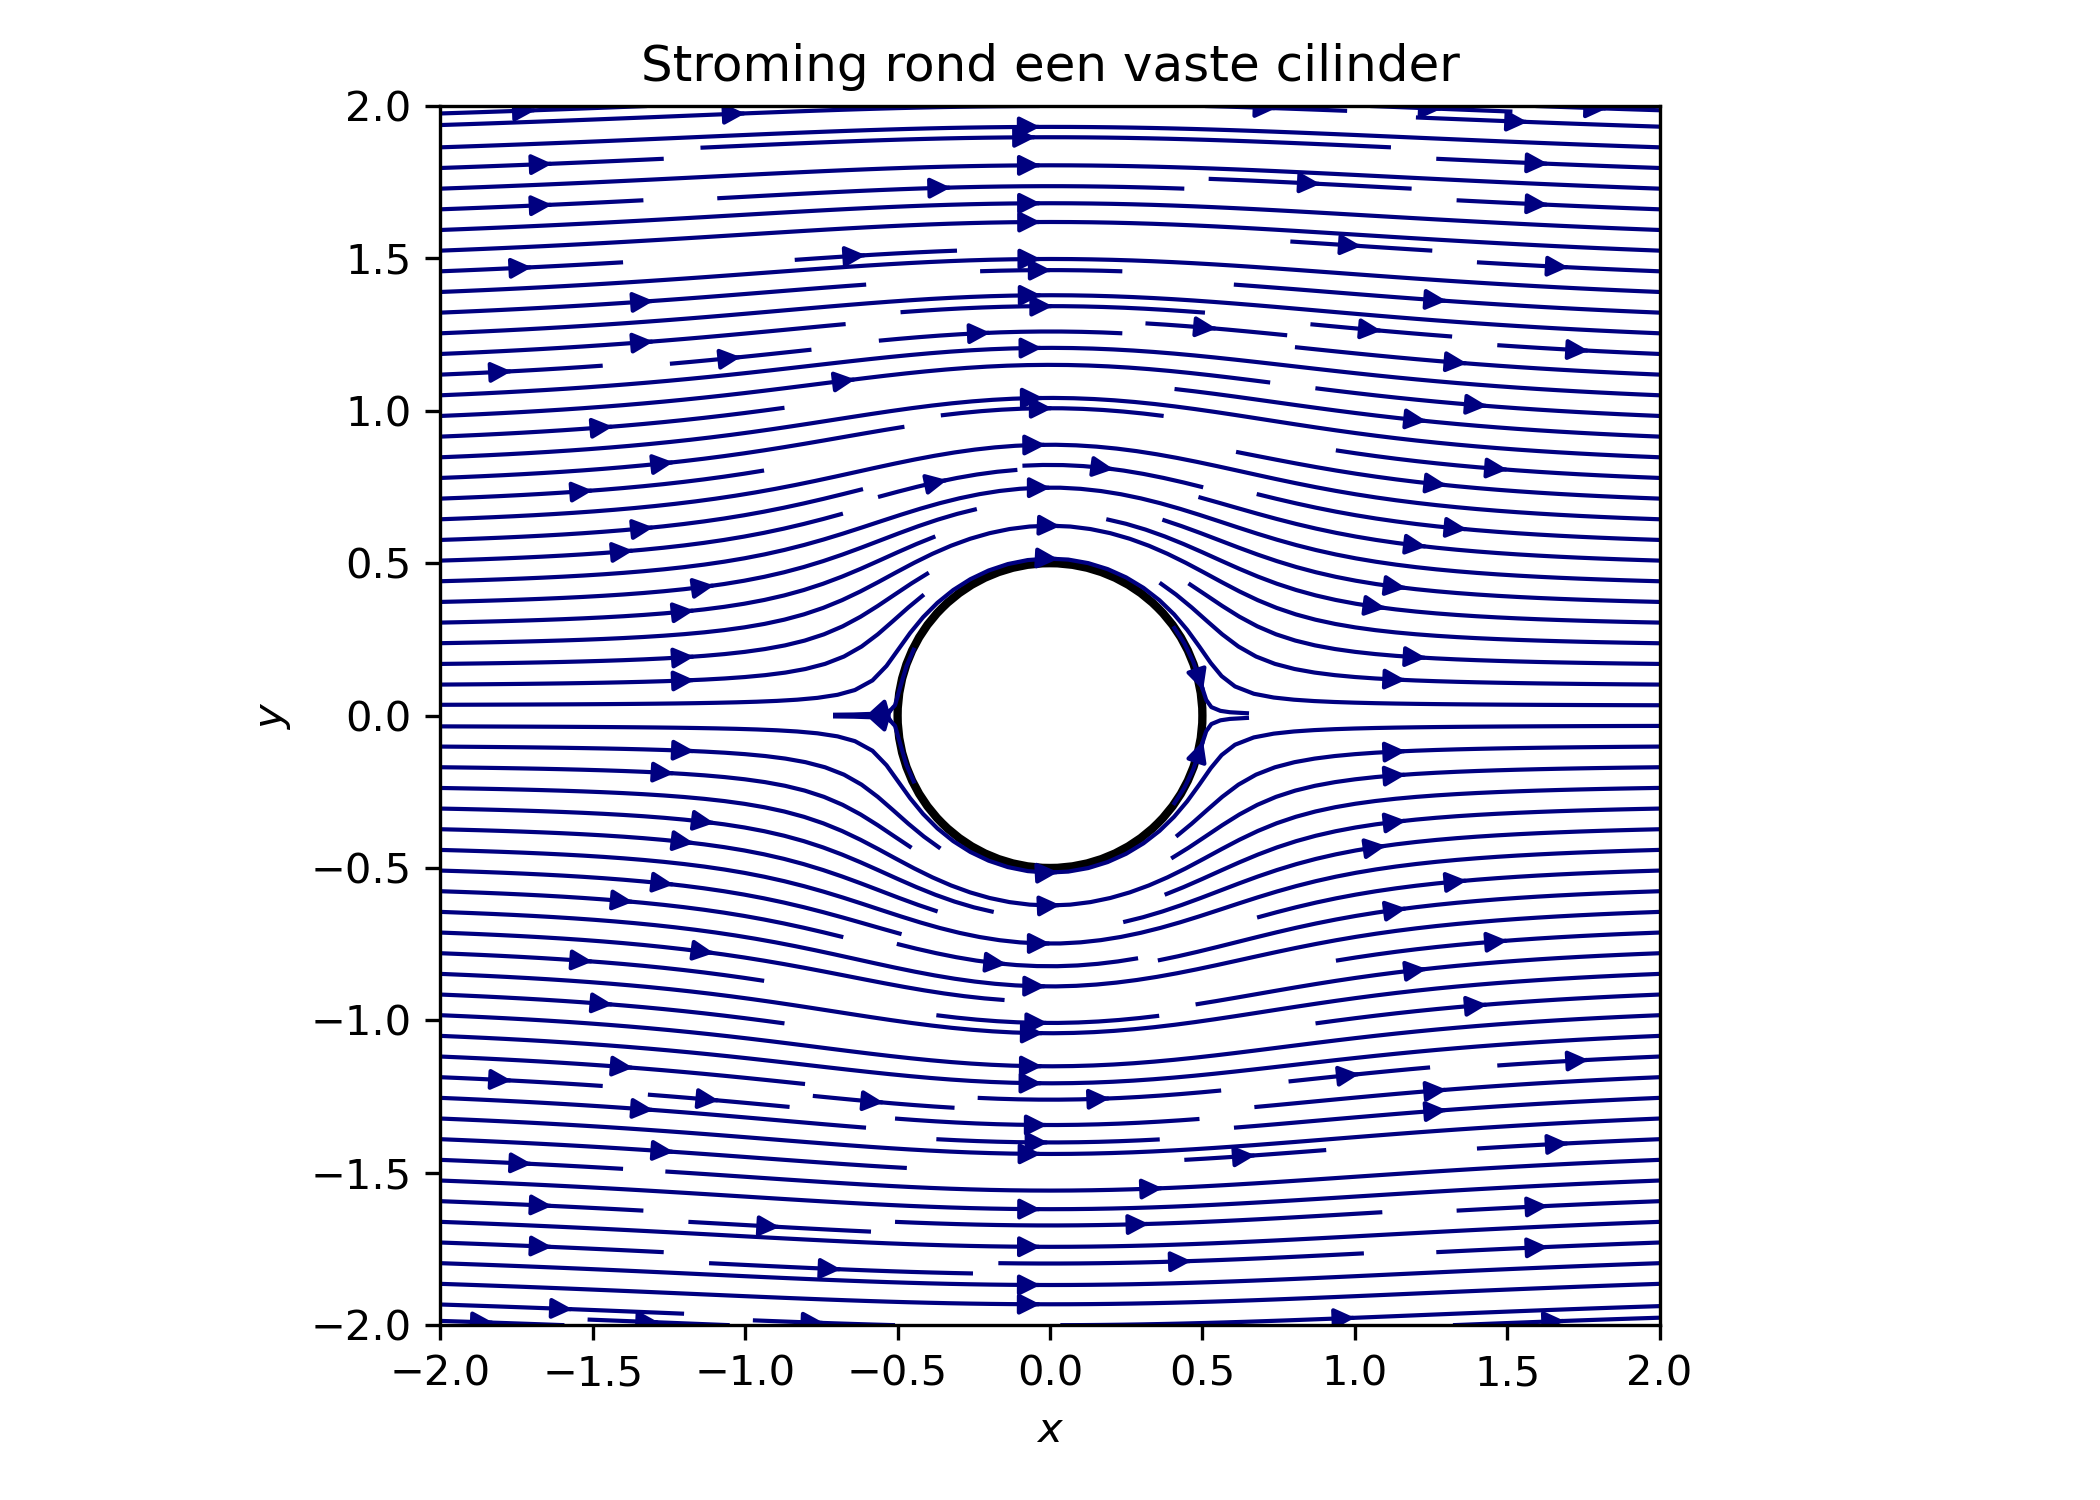
\includegraphics[width=0.85\textwidth]{cylinder_flow}
    \caption{}
    \label{fig:cylinderflow}
\end{figure}

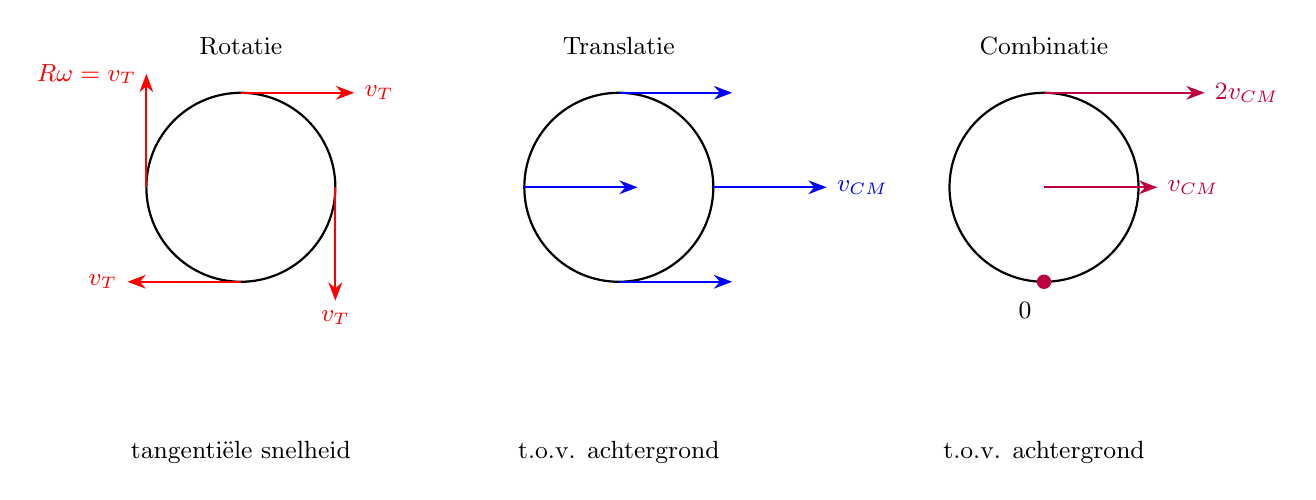
\begin{tikzpicture}[scale=1.2, >=Stealth, every node/.style={font=\small}]

% First: Pure Rotation
    \node at (-3,2.5) {Rotatie};
    \draw[thick] (-3,1) circle (1);
    \draw[->, red, thick] (-4,1) -- (-4,2.2) node[left] {$R\omega = v_T$};
    \draw[->, red, thick] (-3,2) -- (-1.8,2) node[right] {$v_T$};
    \draw[->, red, thick] (-3,0) -- (-4.2,0) node[left] {$v_T$};
    \draw[->, red, thick] (-2,1) -- (-2,-0.2) node[below] {$v_T$};

% Second: Pure Translation
    \node at (1,2.5) {Translatie};
    \draw[thick] (1,1) circle (1);

    \draw[->, blue, thick] (0,1) -- (1.2,1);
    \draw[->, blue, thick] (2,1) -- (3.2,1) node[right] {$v_{CM}$};
    \draw[->, blue, thick] (1,0) -- (2.2,0);
    \draw[->, blue, thick] (1,2) -- (2.2,2);

% Third: Combined Motion
    \node at (5.5,2.5) {Combinatie};
    \draw[thick] (5.5,1) circle (1);
    \draw[->, thick, purple] (5.5,2) -- (7.2,2) node[right] {$2v_{CM}$};
    \draw[->, thick, purple] (5.5,1) -- (6.7,1) node[right] {$v_{CM}$};
    \filldraw[purple] (5.5,0) circle (2pt);
    \node at (5.3,-0.3) {$0$};

% Labels
    \node[align=center] at (-3,-1.8) {tangentiële snelheid};
    \node[align=center] at (1,-1.8) {t.o.v. achtergrond};
    \node[align=center] at (5.5,-1.8) {t.o.v. achtergrond};

\end{tikzpicture}






\begin{figure}[htbp]
    \centering
    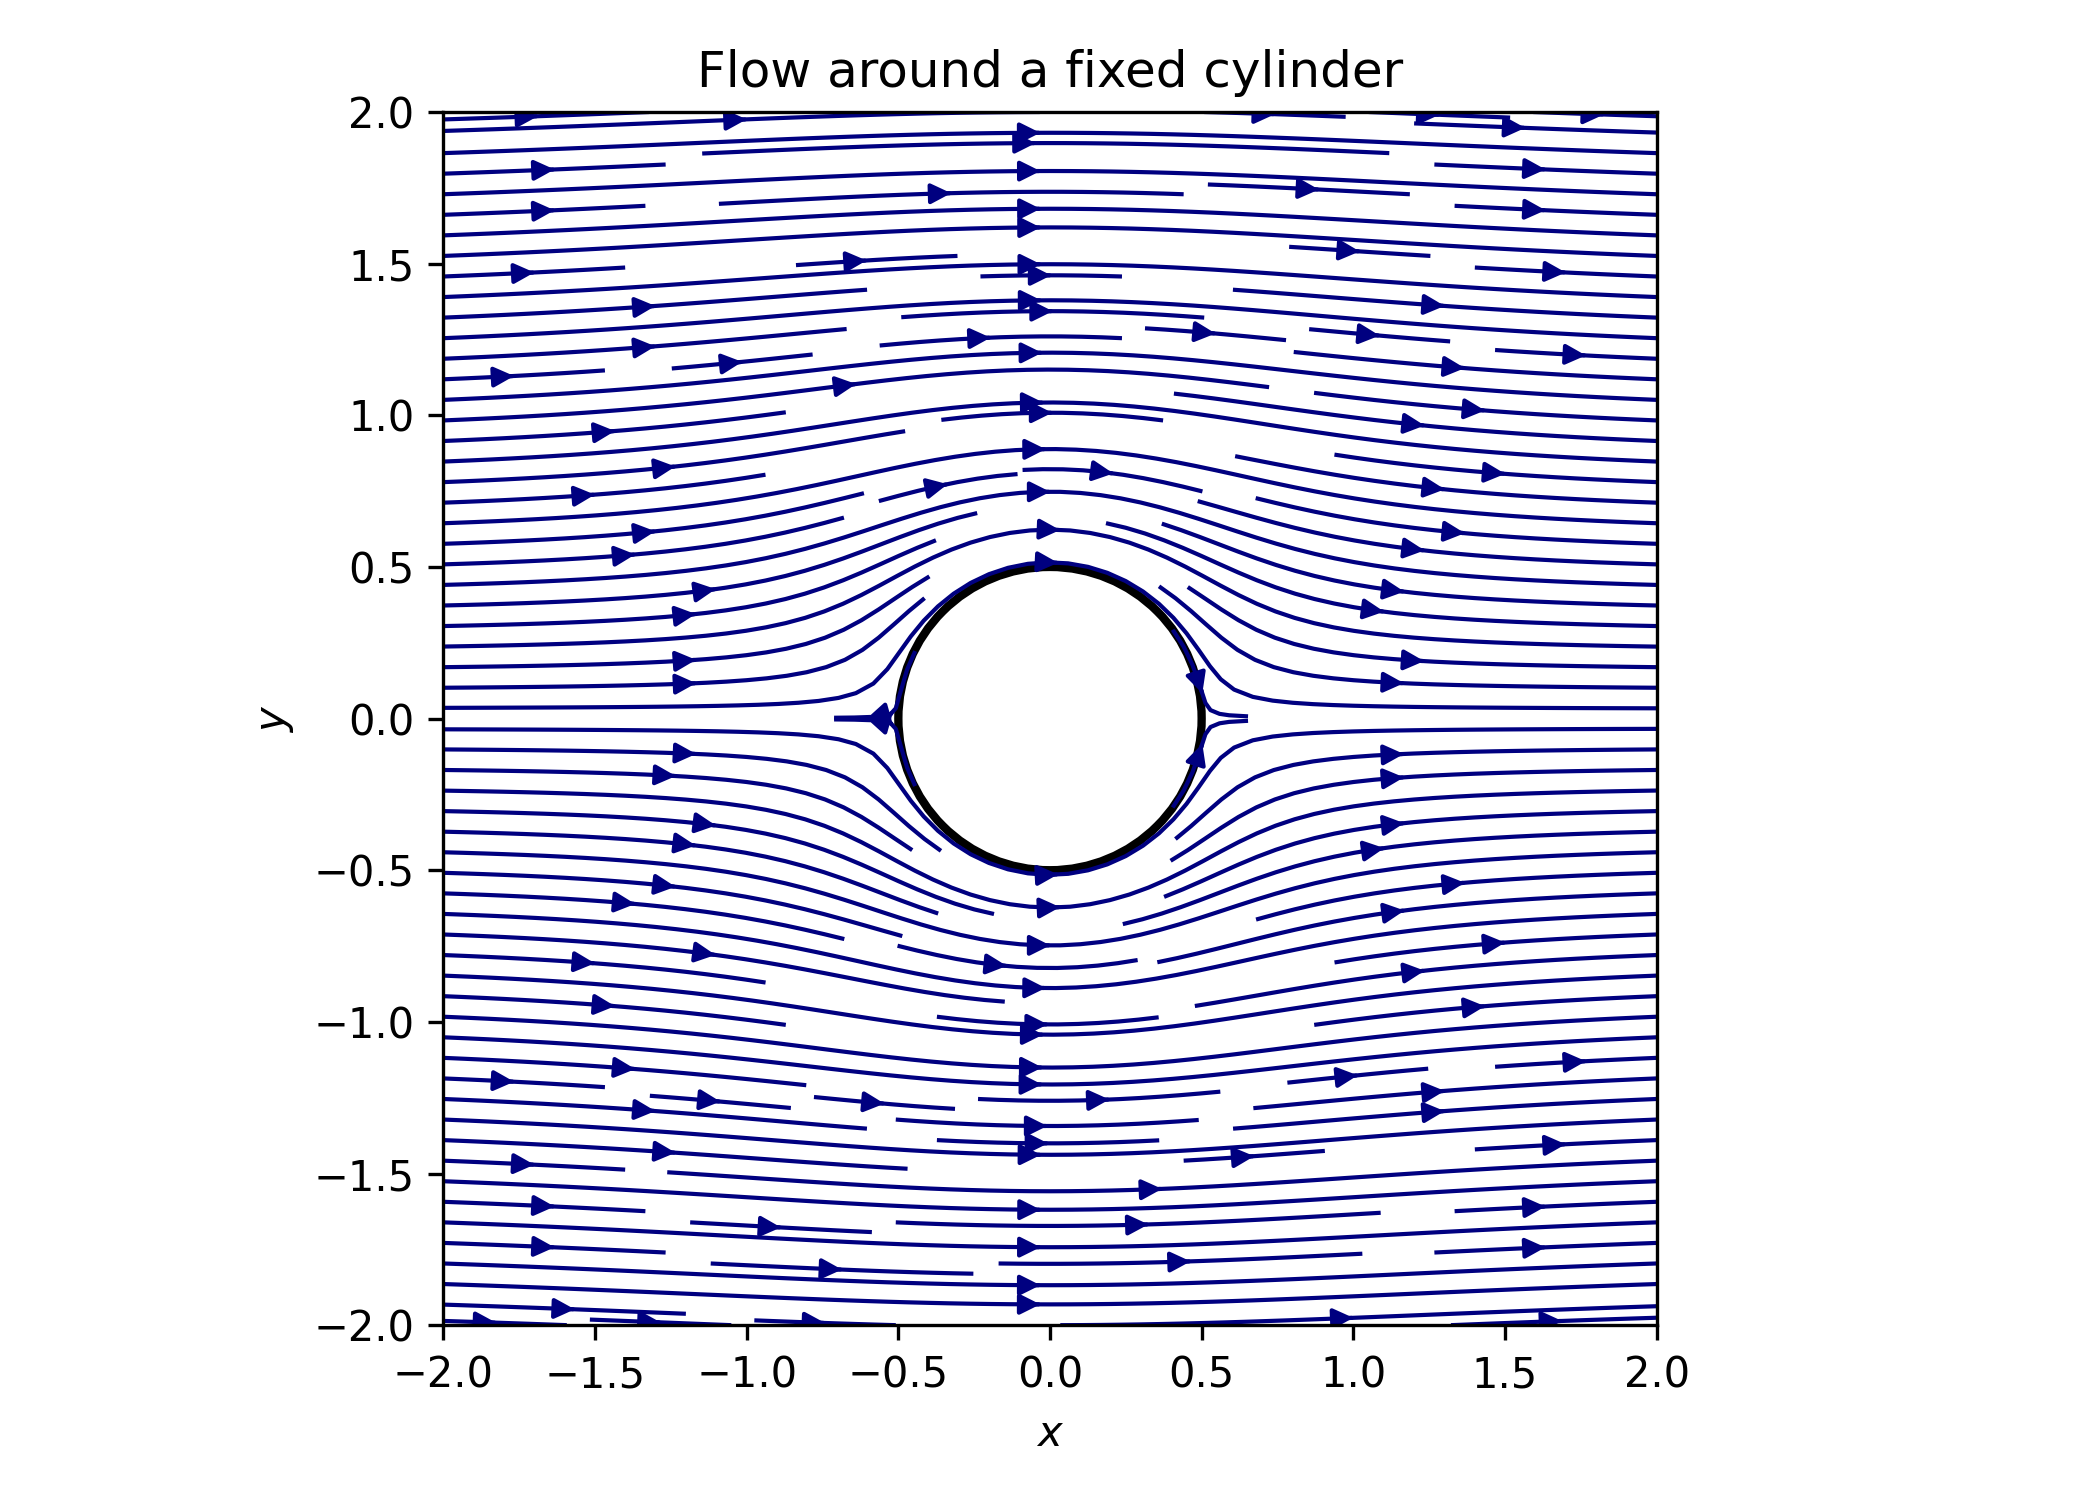
\includegraphics[width=0.85\textwidth]{02_cylinder_flow}
    \caption{Visualisatie van stroming rond een vaste cilinder als analogie voor ætherstroming rond een stabiele wervel in het æthermodel. De uniforme achtergrondstroom wordt lokaal vervormd door de aanwezigheid van de wervelstructuur. Dit klassieke potentiaalstroomprofiel vormt de basis voor latere interpretaties van ætherinteracties in het model.}
    \label{fig:cylinderflow}
\end{figure}

\section{Introductie}
In een moderne heropleving van Lord Kelvins wervel-atoomhypothese uit 1867~\cite{Kelvin1867-vortex} beschouwen we een absolute Euclidische ruimte gevuld met een supervloeibare æther. In dit kader zijn elementaire deeltjes (atomen) stabiele wervelknopen in de æther, en \emph{tijd} wordt geïdentificeerd met de intrinsieke hoekrotatie van deze wervelkernen. De uitdaging is om \emph{tijdsdilatatie}-formules af te leiden die analoog zijn aan die in de speciale en algemene relativiteitstheorie (SR en GR), met behulp van fysieke parameters van de æther (zoals constante dichtheid en fundamentele schalen zoals de Planck-tijd) in plaats van 4D-ruimtetijdgeometrie. We vereisen dat elke nieuwe formule gevestigde relativistische effecten reproduceert - bijvoorbeeld het vertragen van klokken in de buurt van een massief lichaam (gravitationele roodverschuiving) of bij hoge snelheid (speciaal-relativistische tijdsdilatatie) - ondanks het werken in een vlakke 3D-achtergrond.Met andere woorden, de \emph{werveldynamica} van de æther — zoals geïllustreerd in Figuur~\ref{fig:cylinderflow} — moet de 4D-metrische kromming van GR met hoge precisie nabootsen.


Dit rapport ontwikkelt een wiskundig rigoureus model voor tijdsdilatatie in het superfluïde ætherparadigma. We beginnen met het formaliseren van
de belangrijkste aannames van het æthermodel en definiëren hoe de rotatie van een wervel als een fysieke klok dient. Vervolgens leiden we twee
sets tijdsdilatatievergelijkingen af: één voor relatieve beweging (analoog aan SR) en één voor gravitatievelden (analoog aan GR). Tot slot laten we zien dat deze resultaten overeenkomen met standaard relativistische voorspellingen (bijv. gravitationele roodverschuiving, orbitale kloksnelheden) en bespreken we hoe \emph{wervelhoeksnelheid} in de æther de ruimtetijdkromming vervangt als het mechanisme van tijdsdilatatie. We citeren primaire literatuur ter vergelijking en validatie en gebruiken fundamentele constanten (Planck-tijd $t_\textrm{P}$, maximale kracht $F_{\max}$, ætherdichtheid $\rho_{\text{\ae}}$, enz.) om de nieuwe formules in vertrouwde termen uit te drukken.
\section{Superfluïde Æther Framework}

We veronderstellen een stationaire, Euclidische 3-dimensionale æther die zich gedraagt als een superfluïde met een viscositeit van nul en een constante massadichtheid. Dit continue medium vormt de basis van alle natuurkunde: deeltjes zijn topologische wervelstructuren in de æther en velden corresponderen met stromingspatronen (vorticiteit, druk, etc.). De belangrijkste aannames kunnen als volgt worden samengevat:

\begin{itemize}
    \item \textbf{Platte absolute ruimte:} Ruimte is een vaste Euclidische achtergrond (geen inherente kromming). Er is een voorkeursrustframe gedefinieerd door de æther in rust. (Dit is vergelijkbaar met Lorentz's oorspronkelijke absolute frameconcept, maar nu met een fysieke superfluïde die de ruimte vult~\cite{Winterberg2002-PlanckAether}). Alle coördinaatafstanden worden gemeten in deze vlakke ruimte, niet in een gebogen metriek.

    \item \textbf{Constante dichtheid:} De æther heeft een uniforme dichtheid $\rho_{\text{\ae}}$ en is onsamendrukbaar (analoog aan supervloeibaar helium bij $T=0$). Daarom kunnen æthervolume-elementen niet worden gecreëerd of vernietigd; de stroming is divergentieloos, behalve mogelijk bij singuliere wervelkernen. Alle lokale variaties (bijv. nabij massa's) hebben betrekking op snelheidsvelden of druk, niet op dichtheidsveranderingen.

    \item \textbf{Atomen als wervelknopen:} Volgens Kelvin~\cite{Kelvin1867-vortex} is een "atoom" of fundamenteel deeltje een gekwantiseerde wervellus of -knoop in de æther. Het heeft een goed gedefinieerde kern (van de orde van de Planck-lengte $l_{\textrm P}$ in straal, volgens de Planck-æther-theorieën~\cite{Winterberg2002-PlanckAether}) waar æther circulair omheen stroomt. De topologie van de wervel (knooptype) zou kunnen overeenkomen met het type deeltje, terwijl de intrinsieke hoeksnelheid $\omega$ (de wervelsnelheid van æther rond de kern) het deeltje zijn interne klok geeft.

    \item \textbf{Tijd als wervelrotatie:} De juiste tijd voor een deeltje wordt gedefinieerd door de rotatie van zijn wervelkern. Bijvoorbeeld, een bepaalde vaste rotatiehoek (zeg één volledige $2\pi$ omwenteling van de kern) zou een vaste hoeveelheid juiste tijd kunnen definiëren (misschien in de orde van één "tik"). De leeftijd of interne tijd van een deeltje gaat vooruit met het aantal omwentelingen dat zijn kern uitvoert. Snellere kernrotatie betekent een snellere interne tijdssnelheid. Belangrijk is dat deze rotatie een absoluut fysiek proces is dat plaatsvindt ten opzichte van de æther.

    \item \textbf{Opkomende temperatuur en irrotationele stroming:} In het grootste deel van de æther (ver van wervelkernen) kan de stroming irrotationeel en laminair zijn. Macroscopische thermodynamische concepten (temperatuur, entropie) worden statistisch gezien verondersteld voort te komen uit kleinschalige ætherdynamica, maar op fundamenteel niveau is de æther een dissipatieloos, niet-thermisch medium. Daarom negeren we alle eindige-temperatuur- of viskeuze effecten – de æther is een perfecte niet-viskeuze vloeistof.

    \item \textbf{Vorticiteitsvelden en interacties:} Alle krachten (elektromagnetisme, zwaartekracht, enz.) worden gemedieerd door ætherstromen.
    Ruimtelijke gradiënten in vorticiteit of heliciteit (draaiing van wervellijnen) in het ætherveld kunnen andere vortices beïnvloeden.
    Bijvoorbeeld, wat wij waarnemen als een $\text{"zwaartekrachtsveld"}$ zal worden gemodelleerd door een bepaald æthersnelheidsveld (zoals we later
zullen toelichten). Het principe van maximale kracht $ F_\text{\max} = c^4 / 4 G $ uit de algemene relativiteitstheorie~
    \cite{Schiller2022-maxforce}, dat een bovengrens stelt aan kracht in de natuur, wordt verondersteld voort te komen uit de eigenschappen van de æther (bijv. maximale stroomsnelheid $c$ en dichtheid $\rho_\text{\ae}$ leggen een limiet op aan impulsflux/kracht).
\end{itemize}

Binnen dit raamwerk biedt de æther een absolute referentie voor beweging, maar alle meetbare effecten moeten uiteindelijk consistent zijn met de relativiteitstheorie. Zoals Winterberg (2002) het formuleerde, ``kan het universum worden beschouwd als Euclidische vlakke ruimtetijd, op voorwaarde dat we een dichtbevolkt kwantumvacuüm superfluïde als æther opnemen''~\cite{Winterberg2002-PlanckAether}.


\begin{figure}[htbp]
    \centering
    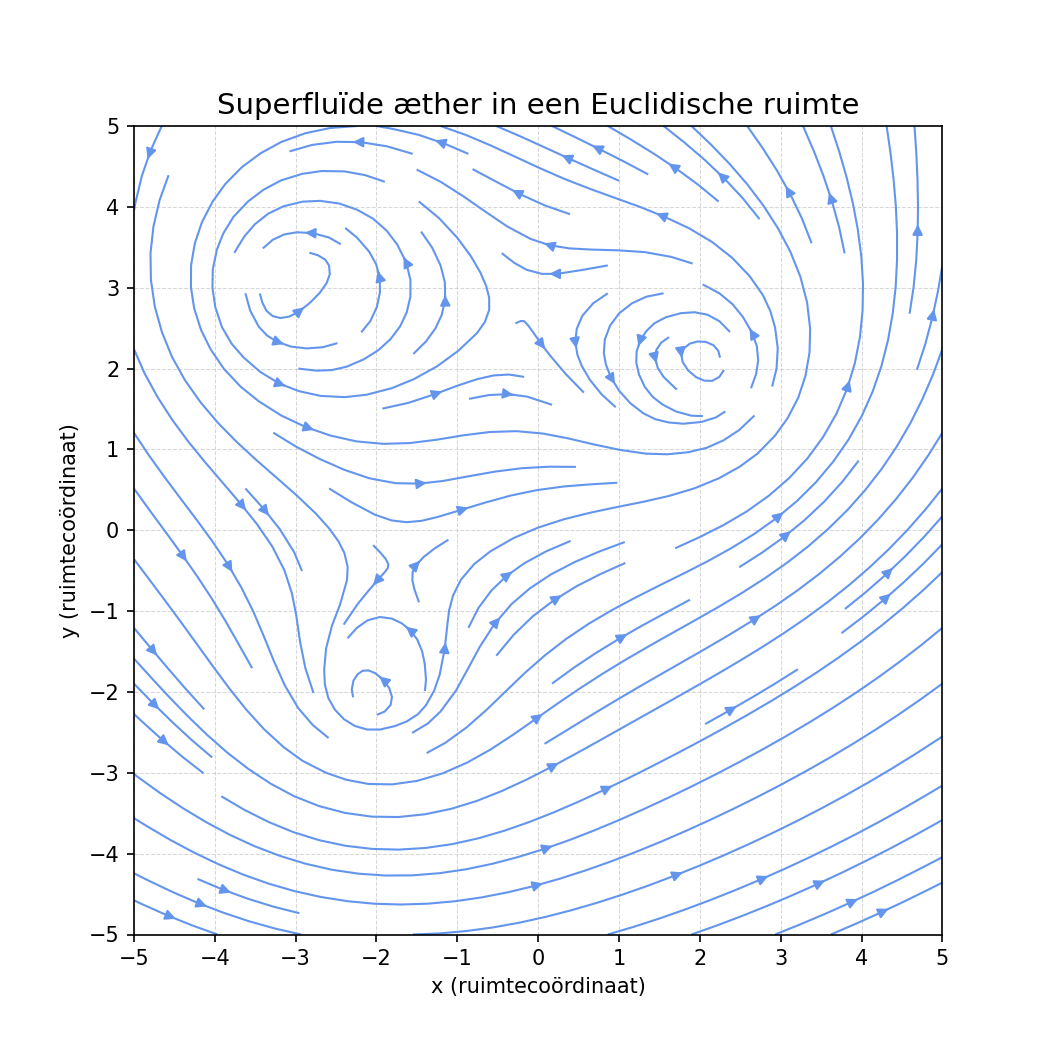
\includegraphics[width=0.85\textwidth]{2-ÆtherSuperfluïde}
    \caption{.}
    \label{fig:ÆtherSuperfluïde}
\end{figure}


\textbf{Definities en constanten:} Voor later gebruik definiëren we enkele fundamentele constanten in dit model. De Planck-tijd is
\[
    t_{\textrm P} = \sqrt{\frac{\hbar G}{c^5}} \approx 5.39\times10^{-44}\ \text{s},
\]
de natuurlijke eenheid van tijd in kwantumzwaartekracht. Het vertegenwoordigt ongeveer de tijd die licht nodig heeft om één Planck-lengte $l_{\textrm P} \approx 1.62\times10^{-35}$ m af te leggen. In veel superfluïde-æther-theorieën zou $l_{\textrm P}$ de kerndiameter van elementaire wervelstructuren kunnen zijn~\cite{Winterberg2002-PlanckAether}, dus één volledige rotatie van een elementaire wervelstructuur met de lichtsnelheid $c$ zou de orde van $t_{\textrm P}$ aannemen. Dus $t_{\textrm P}$ stelt een bovengrens in voor de rotatiefrequentie ($\sim 10^{43}$ s$^{-1}$) voor elke fysieke klok in de æther.

Een andere nuttige constante is de voorgestelde maximale kracht:
\[
    F_\text{\max} = \frac{c^4}{4G} \approx 3.0\times10^{43}\ \text{N}.
\]
Dit verschijnt als een bovengrens in de algemene relativiteitstheorie~\cite{Schiller2022-maxforce}, bijvoorbeeld, de zwaartekracht tussen twee zwarte gaten kan $F_\text{\max}$ niet overschrijden. In de æther-afbeelding kan $F_{\textrm max}$ worden geïnterpreteerd als de maximale spanning of sleepkracht die de superfluïde æther kan verdragen wanneer stromingen de lichtsnelheid naderen.

We behouden $c$ (snelheid van het licht in vacuüm) als de karakteristieke signaalsnelheid in de æther (bijv. de snelheid van geluid of golfvoortplanting in het superfluïde vacuüm, vaak genomen als $c = \sqrt{B/\rho_{\text{\ae}}}$ voor bulkmodulus $B$). De Newtoniaanse gravitatieconstante $G$ zal ingaan bij het koppelen van ætherstroming aan massa (aangezien massa in wezen een wervel is met een bepaalde circulatie en kernstructuur die verband houdt met $G$). We zullen indien nodig extra constanten introduceren.
\section{Wervelklokken en juiste tijd}

\begin{figure}[H]
    \centering
    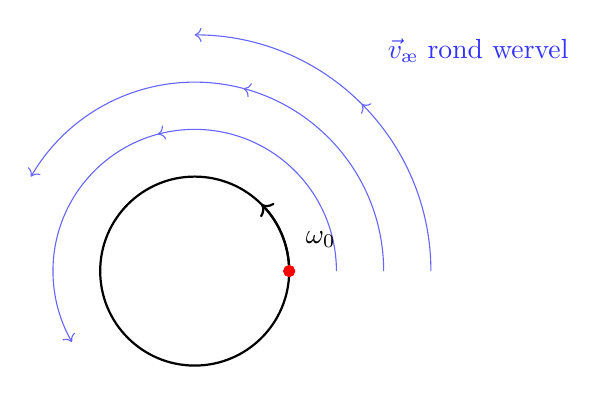
\begin{tikzpicture}[scale=2]
        \usetikzlibrary{decorations.markings}

        % Streamlines with varying arc lengths
        \draw[blue!60, ->,
            postaction={decorate},
            decoration={markings,
            mark=at position 0.5 with {\arrow{>}}}
        ] (0.9,0) arc (0:210:0.9); % Short arc

        \draw[blue!60, ->,
            postaction={decorate},
            decoration={markings,
            mark=at position 0.5 with {\arrow{>}}}
        ] (1.2,0) arc (0:150:1.2); % Medium arc

        \draw[blue!60, ->,
            postaction={decorate},
            decoration={markings,
            mark=at position 0.5 with {\arrow{>}}}
        ] (1.5,0) arc (0:90:1.5); % Long arc

        % Vortexring
        \draw[thick] (0,0) circle (0.6);
        \draw[thick, ->] (0:0.6) arc (0:45:0.6);
        \node at (0.8,0.2) {$\omega_0$};
        \filldraw[red] (0.6,0) circle (1pt);

        % Vectorveld label
        \node[blue!80] at (1.8,1.4) {$\vec{v}_{\ae}$ rond wervel};

    \end{tikzpicture}
    \caption{Elke $2\pi$ rotatie van de wervelkern = één tick van de interne klok.}
    \label{fig:wervelklok}
\end{figure}

In dit model wordt een klok gerealiseerd door de rotatie van een microscopische wervel. Om dit concreet te maken, beschouw een vrij deeltje in
rust in de æther. Zijn wervelkern draait gestaag en sleept de nabijgelegen æther rond. Laat $\omega_0$ de hoeksnelheid van deze kern  aanduiden, gemeten in het æther-rustframe (in eenheden radialen per seconde). Per definitie is $\omega_0$ de \emph{juiste rotatiefrequentie} van het deeltje, overeenkomend met zijn juiste tijd $\tau$.

We kunnen $\omega_0$ relateren aan het verstrijken van de juiste tijd: als de kern in een interval met $\Delta \theta$ radialen roteert, dan is de verstreken juiste tijd
\[
    \Delta \tau = \frac{\Delta \theta}{\omega_0} \,.
\]
Als we bijvoorbeeld $2\pi$ radialen van rotatie kiezen als een \("\)tik\("\) van de klok, dan is de juiste periode $T_0 = 2\pi/\omega_0$. Men zou zich kunnen voorstellen dat $\omega_0$ wordt bepaald door de interne structuur van het deeltje - bijvoorbeeld, de wervel van een proton zou kunnen roteren met ongeveer $10^{23}$ rad/s zodat $T_0 \sim 10^{-23}$ s voor één omwenteling (dit is speculatief, maar opmerkelijk genoeg stelde de Broglie in 1924 voor dat elk deeltje met rustmassa $m$ een interne klok heeft met frequentie $mc^2/h$~\cite{deBroglie1924-frequency}, in de orde van $10^{21}$ Hz voor een elektron; een wervelmodel zou een fysieke oorsprong kunnen bieden voor deze \emph{Zitterbewegung} frequentie als kernrotatie).

Voor nu is $\omega_0$ een vrije parameter die de kloksnelheid in rust weergeeft. Wanneer het deeltje niet vrij is of niet in rust is, kan de waargenomen rotatiesnelheid veranderen. We definiëren $\omega_{\textrm obs}$ als de hoeksnelheid van de wervelkern zoals waargenomen door een statische ætherframe-waarnemer (d.w.z. een in rust ten opzichte van de æther) onder welke omstandigheden dan ook (beweging of zwaartekracht). De verhouding $\omega_{\textrm obs}/\omega_0$ geeft dan de snelheid van de klok ten opzichte van de juiste tijd.

In feite, aangezien $\Delta \tau = \Delta \theta / \omega_0$ altijd geldt voor de klok zelf, en $\Delta t$ (coördinaattijd) overeenkomt met $\Delta \theta / \omega_{\textrm obs}$ (de hoek gedraaid in labframetijd), hebben we:
\[
    \frac{\Delta \tau}{\Delta t} = \frac{\Delta \theta / \omega_0}{\Delta \theta / \omega_{\textrm obs}} = \frac{\omega_{\textrm obs}}{\omega_0} \,. \tag{1}
\]

Deze belangrijke relatie koppelt de fysieke vertraging van de spin $\omega_{\textrm obs}$ van de wervel aan de tijdsdilatatiefactor. Als $\omega_{\textrm obs} < \omega_0$, loopt de klok langzaam (aangezien $\Delta \tau < \Delta t$).

Onze taak in de volgende secties is om $\omega_{\textrm obs}$ te bepalen voor twee gevallen:
\begin{enumerate}
    \item Wanneer de wervel (deeltje) met snelheid $v$ door de æther beweegt,
    \item Wanneer de wervel zich in een gravitatiepotentiaal (ætherstroom) bevindt die wordt gecreëerd door een massief lichaam.
\end{enumerate}
We zullen ontdekken dat $\omega_{\textrm obs}/\omega_0$ in deze gevallen respectievelijk de bekende Lorentz- en gravitationele tijdsdilatatiefactoren reproduceert.

Voordat we verdergaan, benadrukken we dat \emph{eigen tijd $\tau$ in dit model fundamenteel slechts een telling is van de rotatie van de wervel}. Dit biedt een objectief, mechanistisch beeld van tijd: bijvoorbeeld, je zou je een klein vlaggetje of markering op de wervelkern kunnen voorstellen die rondjes rond de kern voltooit – elke ronde is een ondubbelzinnige fysieke gebeurtenis die overeenkomt met een vaste hoeveelheid eigen tijd. Verschillende fysieke klokken (atomen, moleculen, etc.) zouden uiteindelijk allemaal hun tijd traceren naar zulke microscopische circulaties in de universele æther.

Voor een bespreking van hoe samengestelde klokken bestaande uit meerdere wervelknopen collectief tijdsdilatatie ondervinden, zie Appendix~\ref{appendix:KlokkenInWervelstructuren}.

Zolang de natuurkundige wetten zodanig zijn dat deze circulaties stabiel en identiek zijn voor identieke deeltjes, biedt dit een standaard van tijd. Vervolgens laten we zien hoe beweging door de æther en ætherstromen $\omega_{\textrm obs}$ beïnvloeden.
\section{Tijdsdilatatie door relatieve beweging}

Beschouw eerst de tijdsdilatatie voor een deeltje dat met hoge snelheid beweegt ten opzichte van het æther-rustframe. Empirisch weten we dat een klok die met snelheid $v$ beweegt, tijd ervaart die langzamer is met de Lorentz-factor $\gamma = 1/\sqrt{1 - v^2/c^2}$. In dit model leiden we hetzelfde effect af door de invloed van absolute æther-beweging op de rotatie van de wervelkern te analyseren.

\subsection*{(a) Kinematische afleiding}

Laat een wervel in rust zijn in zijn eigen frame $S'$ maar met snelheid $v$ bewegen ten opzichte van het æther-rustframe $S$. In $S'$ roteert de wervel met hoekfrequentie $\omega_0$ en definieert de juiste tijd $\tau$. Door Lorentz-tijddilatatie ziet een waarnemer in $S$ de klok vertragen:
\[
    \omega_{\text{obs}} = \omega_0 \sqrt{1 - \frac{v^2}{c^2}} \,.
\]
Vanuit de relatie tussen eigentijd en coördinatentijd,
\[
    \frac{d\tau}{dt} = \frac{\omega_{\text{obs}}}{\omega_0} = \sqrt{1 - \frac{v^2}{c^2}} \,. \tag{2}
\]

Dit komt overeen met de standaard SR-tijddilatatieformule. In ons model is het fysieke mechanisme dat etherbeweging over de wervel de wervelsnelheid verstoort, waardoor de schijnbare rotatie in het etherframe wordt vertraagd.

\subsection*{(b) Vloeistofdynamische interpretatie}

Een complementaire interpretatie gebruikt analogieën van samendrukbare stroming. In de vloeistofdynamica ervaart een lichaam dat met snelheid $v$ beweegt in een samendrukbaar medium met signaalsnelheid $c$ vervormingen evenredig aan $\gamma = 1/\sqrt{1 - v^2/c^2}$. Dit kan worden gezien als een Doppler-tijddilatatie of weerstand tegen het handhaven van coherente circulatie.

Naarmate de snelheid de æthersignaalsnelheid $c$ nadert, comprimeert de omringende stroming en biedt weerstand aan wervelrotatie. Daarom daalt de hoeksnelheid die in het ætherframe wordt gezien, en:
\[
    \omega_{\text{obs}} = \omega_0 \sqrt{1 - \frac{v^2}{c^2}} \Rightarrow \frac{d\tau}{dt} = \sqrt{1 - \frac{v^2}{c^2}} \,. \tag{3}
\]

\subsection*{Implication}

Dit geeft ons de relativistische tijdsdilatatie voor een bewegende klok:
\[
    \boxed{\frac{d\tau}{dt} = \sqrt{1 - \frac{v^2}{c^2}}}
\]
binnen een Euclidische, æther-gebaseerde vlakke ruimte, en komt overeen met alle speciale relativiteitstheorie-experimentele voorspellingen~\cite{Rado2020-aether-Lorentz,Levy2009-aether-clock}.
\section{Gravitationel Tijd Dilatatie}

In de algemene relativiteitstheorie lopen klokken dieper in een gravitationele potentiaalput langzamer vergeleken met klokken met hogere potentialen. We reproduceren dit resultaat met behulp van etherstroomvelden in plaats van ruimtetijdkromming.

\subsection*{Ætherstroom als zwaartekracht}

We nemen aan dat massa $M$ een inwaartse radiale stroming van æther induceert. Bij een straal $r$ wordt deze stroomsnelheid gegeven door:
\[
    v_g(r) = \sqrt{\frac{2GM}{r}}.
\]
Dit weerspiegelt de Painlevé-Gullstrand-metriek en het riviermodel van zwarte gaten~\cite{Hamilton2004-river}.

\subsection*{Ætherweerstand en klokvertraging}

Een klok die op straal $r$ in deze inwaartse ætherstroom wordt gehouden, ziet æther er langs bewegen met snelheid $v_g(r)$. De waargenomen hoeksnelheid van de wervelkern wordt daarom verminderd door de weerstand van de ether, net als in het speciale relativiteitsgeval, waarbij beweging door de ether de waargenomen kloksnelheid vermindert.

De gravitationele tijdsdilatatiefactor is dus:
\[
    \frac{d\tau}{dt} = \sqrt{1 - \frac{v_g^2(r)}{c^2}} = \sqrt{1 - \frac{2GM}{rc^2}}. \tag{4}
\]
Dit komt overeen met de Schwarzschild-oplossing voor stationaire waarnemers in de algemene relativiteitstheorie.

\subsection*{Interpretatie}

Deze vergelijking betekent dat hoe dieper een wervel zich in het gravitatiepotentieel bevindt (hoe sneller de lokale etherstroom), hoe langzamer deze roteert vanuit het perspectief van een waarnemer op oneindig. Bij de Schwarzschild-straal $r_s = 2GM/c^2$, $d\tau/dt = 0$: de tijd stopt voor externe waarnemers.

Dit levert een mechanistische interpretatie van gravitationele roodverschuiving op: licht dat wordt uitgezonden door een wervelklok in een sterke potentiaalput, lijkt roodverschoven vanwege de langzamere hoekbeweging van de uitzendende wervel. Het resultaat:
\[
    \boxed{\frac{d\tau}{dt} = \sqrt{1 - \frac{2GM}{rc^2}}}
\]
is volledig consistent met GR en ondersteunt de æther-stroomanalogie~\cite{Schiller2022-maxforce}.
\section{Gecombineerde effecten en verdere voorspellingen}

Nu we afzonderlijke tijdsdilatatiefactoren hebben afgeleid voor beweging door æther en gravitationele ætherstroom, beschouwen we beide effecten nu tegelijkertijd.

\subsection*{Gecombineerde beweging en gravitationeel veld}

Laat een wervelklok bewegen met snelheid $\vec{u}$ in een gebied waar de æther stroomt met snelheid $\vec{v}_g$. De effectieve relatieve snelheid ten opzichte van de lokale ætherstroom is:
\[
    \vec{v}_{\text{rel}} = \vec{u} - \vec{v}_g.
\]
De waargenomen tijdsdilatatie is dan:
\[
    \frac{d\tau}{dt} = \sqrt{1 - \frac{|\vec{v}_{\text{rel}}|^2}{c^2}}. \tag{5}
\]
Deze formulering integreert zowel speciale als algemene relativistische effecten op soepele wijze in één enkele uitdrukking.

\subsection*{Voorbeeld: Circulaire baantijdsdilatatie}

Beschouw een klok die rond een massa $M$ draait met straal $r$. De tangentiële snelheid van de baan is:
\[
    v_{\text{orb}} = \sqrt{\frac{GM}{r}}, \quad v_g(r) = \sqrt{\frac{2GM}{r}}.
\]
Aangezien de baansnelheid loodrecht staat op de radiale ætherinstroom, is de relatieve snelheid:
\[
    v_{\text{rel}} = \sqrt{v_{\text{orb}}^2 + v_g^2} = \sqrt{\frac{3GM}{r}}.
\]

\begin{figure}[htbp]
    \centering
    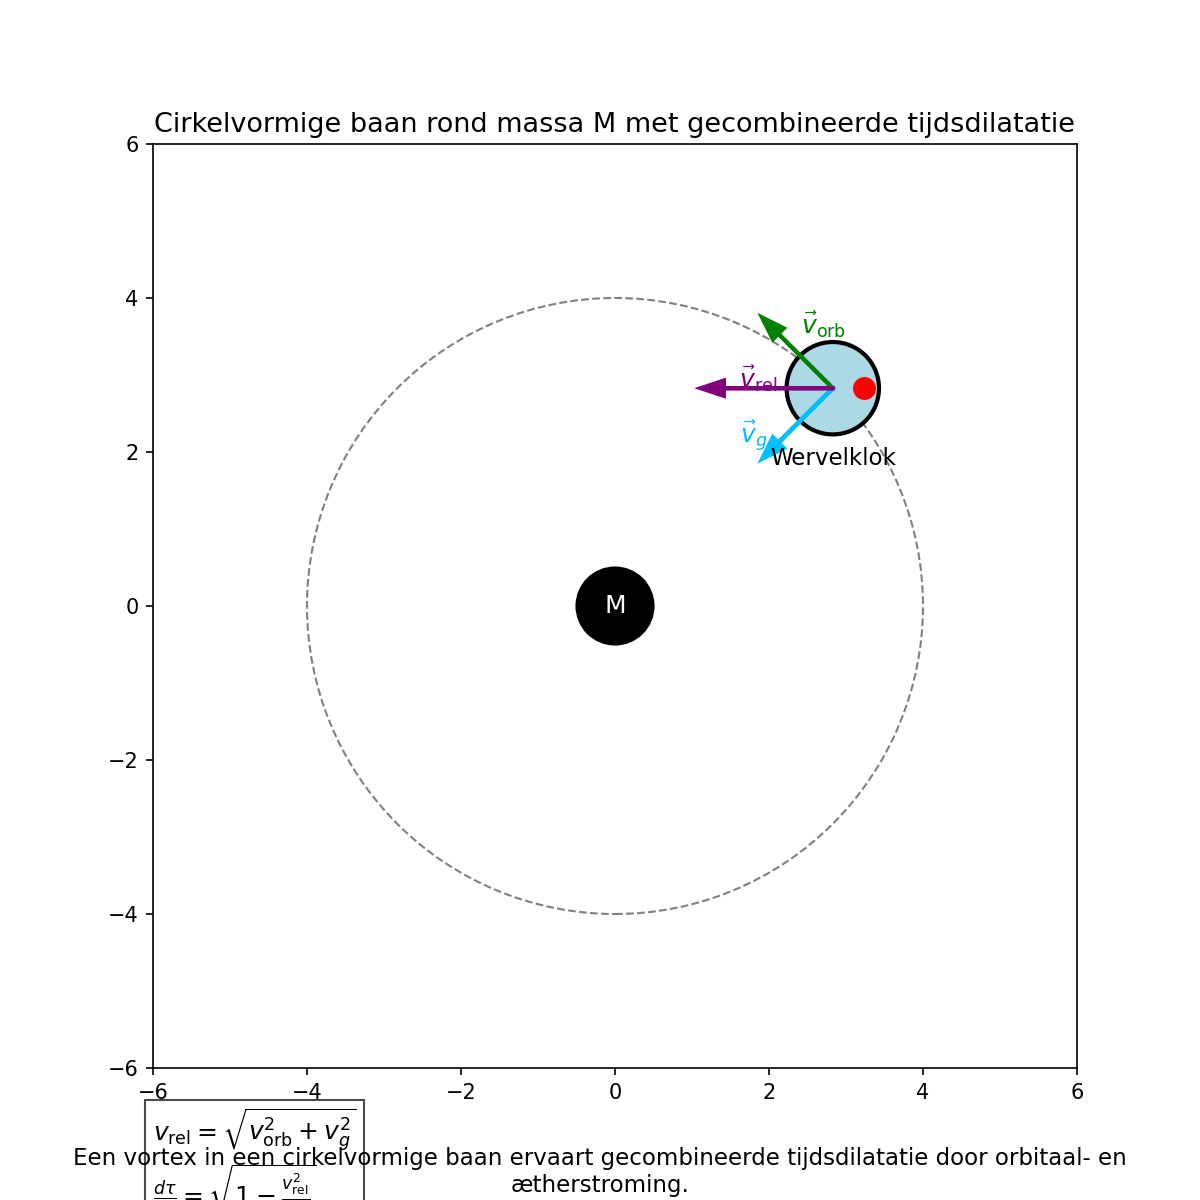
\includegraphics[width=0.85\textwidth]{5-BaanRondMassa}
    \caption{.}
    \label{fig:BaanRondMassa}
\end{figure}


De tijdsdilatatie wordt dus:
\[
    \frac{d\tau}{dt} = \sqrt{1 - \frac{3GM}{rc^2}}. \tag{6}
\]
Dit komt overeen met het exacte resultaat van Schwarzschild-geometrie voor cirkelvormige banen.

\subsection*{Implicaties nabij een horizon}

Als $r \to r_s = 2GM/c^2$ nadert de instroomsnelheid $v_g(r)$ $c$ en vertraagt de klok van elke statische waarnemer tot nul. De ætherstroom onderdrukt de lokale wervelrotatie volledig, wat een natuurlijk mechanisme biedt voor het \("\)bevriezen van de tijd\("\) aan de gebeurtenishorizon.


\begin{figure}[htbp]
    \centering
    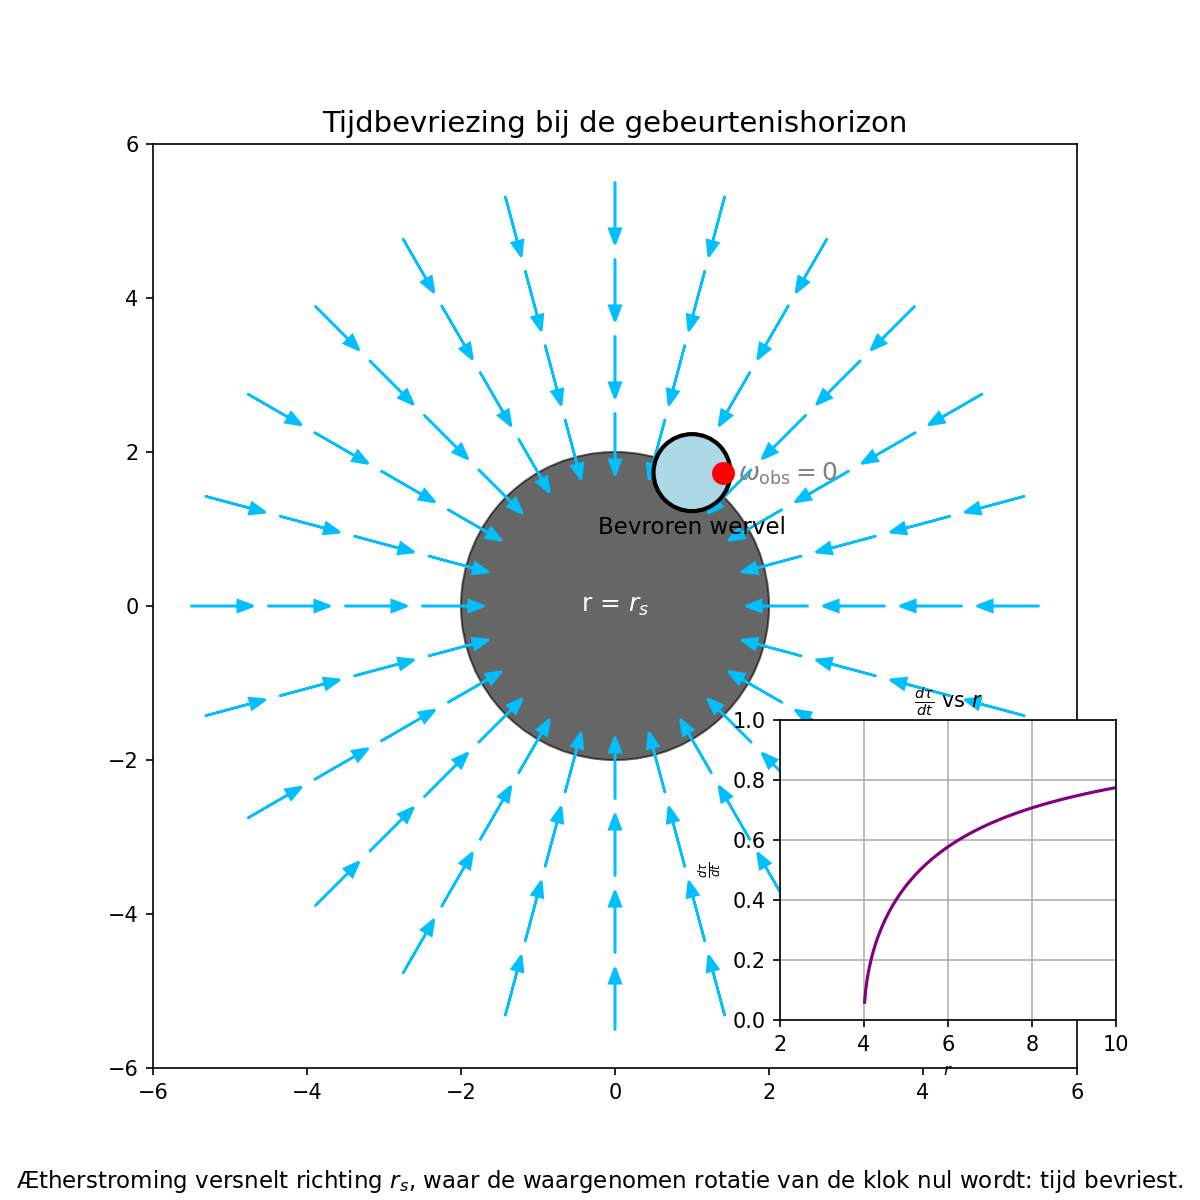
\includegraphics[width=0.85\textwidth]{6-HorizonTijdsbevriezing}
    \caption{.}
    \label{fig:HorizonTijdsbevriezing}
\end{figure}

\subsection*{Uniforme interpretatie}

Dit æthermodel maakt het mogelijk om alle relativistische tijdsdilatatie-effecten te zien als gevolgen van één principe:
\[
    \text{Kloksnelheidsreductie} \;\propto\; \text{relatieve beweging door æther}.
\]
Of deze relatieve beweging nu voortkomt uit traagheidssnelheid of uit ætherische instroom vanwege nabijgelegen massa, het waarneembare gevolg is hetzelfde. Daarom concluderen we:
\[
    \boxed{\frac{d\tau}{dt} = \sqrt{1 - \frac{|\vec{u} - \vec{v}_g|^2}{c^2}}}
\]
als de algemene tijdsdilatatieformule voor het Vortex Æther Model.


\begin{figure}[htbp]
    \centering
    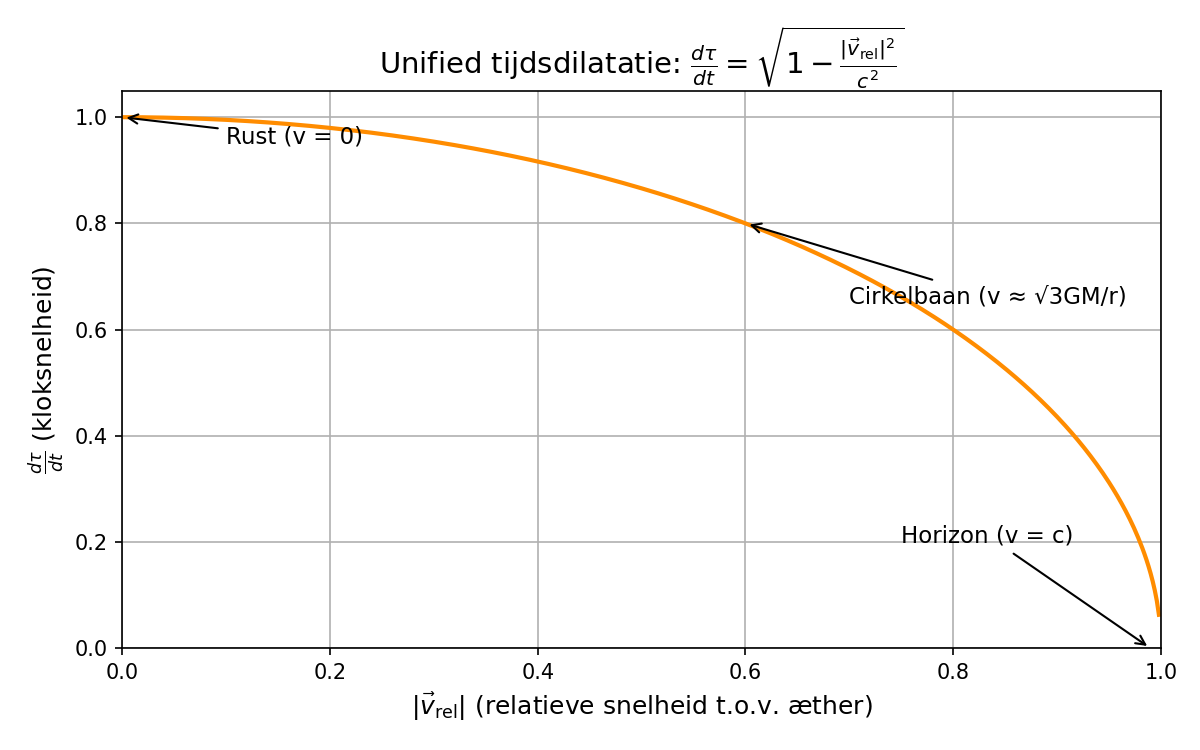
\includegraphics[width=0.85\textwidth]{7-TijdsvertragingRelatieveBeweging}
    \caption{.}
    \label{fig:TijdsvertragingRelatieveBeweging}
\end{figure}

Voor mogelijke experimentele afwijkingen van deze tijdsdilatatieformules t.o.v. de algemene relativiteitstheorie, zie Appendix~\ref{appendix:AfwijkendeVoorspellingen}.
\section{Conclusie}

We hebben tijdsdilatatie-wetten afgeleid binnen een 3D Euclidisch æthermodel, waarbij deeltjes worden gemodelleerd als wervelknopen en tijd wordt gedefinieerd door hun intrinsieke wervelkernrotatie. Beweging door de æther en ætherische instromen (zwaartekrachtvelden) verminderen de waarneembare hoeksnelheid van de wervelrotatie, wat resulteert in:

\begin{itemize}
    \item De speciaal-relativistische tijdsdilatatie:
    \[
        \frac{d\tau}{dt} = \sqrt{1 - \frac{v^2}{c^2}},
    \]
    die voortkomt uit absolute beweging door de æther.

    \item De gravitationele tijdsdilatatie:
    \[
        \frac{d\tau}{dt} = \sqrt{1 - \frac{2GM}{rc^2}},
    \]
    die ontstaat door inwaartse ætherstroom nabij massa $M$.

    \item Het uniforme algemene geval:
    \[
        \frac{d\tau}{dt} = \sqrt{1 - \frac{|\vec{u} - \vec{v}_g|^2}{c^2}},
    \]
    die beweging in een gravitatieveld bestrijkt.
\end{itemize}

Deze resultaten reproduceren nauwkeurig voorspellingen van de speciale en algemene relativiteitstheorie met behulp van fysiek intuïtieve mechanismen die gegrond zijn in vloeistofdynamica.

Het æthermodel elimineert de noodzaak van gekromde ruimtetijd door deze te vervangen door gestructureerde snelheidsvelden in een vlakke ruimte. Het herinterpreteert relativistische tijdseffecten als echte, mechanische gevolgen van wervelkerndynamiek die interageert met een fysieke æther.

Deze benadering koppelt microfysica (wervelkernrotatie) aan kosmologische structuur (horizonten van zwarte gaten) en handhaaft continuïteit over schalen heen. Door tijdsdilatatie te interpreteren als hoekvertraging van wervels, biedt dit model een mechanistisch, veldgebaseerd alternatief voor geometrische ruimtetijdkromming, waarbij experimentele consistentie met SR en GR behouden blijft en tegelijkertijd mogelijkheden worden geopend voor vloeistofdynamische uitbreidingen van fundamentele fysica~\cite{Winterberg2002-PlanckAether,Schiller2022-maxforce}.

Toekomstig werk kan het afleiden van Einsteins veldvergelijkingen van behoud van æthervorticiteit of het testen van laboratoriumanalogen via superfluïde experimenten omvatten. De herinterpretatie van horizonten van zwarte gaten, gravitationele roodverschuiving en kwantumtijdwaarneming via wervelrotatie moedigt dieper theoretisch en experimenteel onderzoek aan naar de rol van de æther in de moderne fysica.

Een uitgebreidere uitwerking van deze ideeën vindt men in het vervolgonderzoek: \textit{“Swirl Clocks and Vorticity-Induced Gravity”} (2025).~\cite{vam2025unified}.

\bibliographystyle{plain}
\bibliography{00_Tijdsdilatatie_in_3D_Superfluïde_Æther_Model}

\end{document}